% !TeX spellcheck = en_GB
\begin{frame}{One-Hot Encoding}
	\begin{itemize}
		\item
		\emphblue{categorical} features common
%		\begin{itemize}
%			\item
%			nominal (e.g.\ colours)
%			
%			\item
%			ordinal (e.g.\ levels of satisfaction)
%		\end{itemize}
	
		\item
		need for numbers in algorithms
	
		\item
		naïve approach: number serially
		\begin{itemize}
			\item
			arbitrary orders
			
			\item
			meaningless arithmetic calculations
		\end{itemize}
	
		\item
		\emphblue{one-hot encoding}
		\begin{itemize}
			\item
			one binary feature for each possible value
		\end{itemize}
	\end{itemize}
	%
	\smallskip
	%
	\begin{center}
		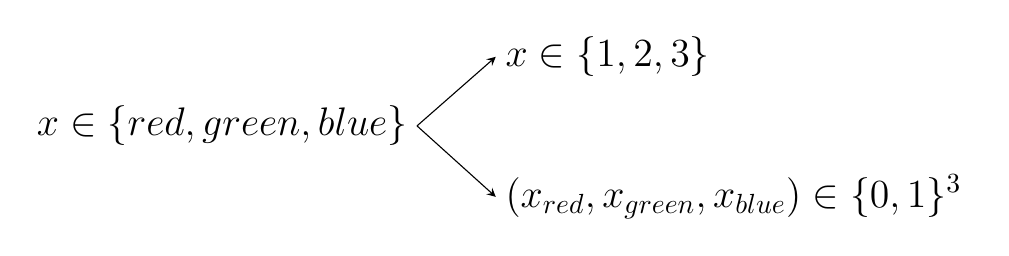
\begin{tikzpicture}[every node/.style={font={\Large}}]
			\node[anchor=east] (a) at (0, 0) {$x \in \{ \text{red}, \text{green}, \text{blue} \}$};
			\node[anchor=south west] (b) at (1, .5) {$x \in \{ 1, 2, 3 \}$};
			\node[red!85!black] (bmark) at (b.east) {\quad \huge \xmark};
			\node[anchor=north west] (c) at (1,-.5) {$(x_{\text{red}}, x_{\text{green}}, x_{\text{blue}}) \in \{ 0, 1 \}^3$};
			\node[green!75!black] (cmark) at (c.east) {\quad \huge \cmark};
			
			\path[-stealth]
			(a.east) edge (b.west) edge (c.west)
			;
		\end{tikzpicture}
	\end{center}
\end{frame}